
\documentclass[10pt]{article}
\usepackage[T1]{fontenc}
\usepackage[utf8]{inputenc}
\usepackage{lmodern}
\usepackage{amsmath,amssymb,mathtools}
\usepackage{tikz}
\usepackage{geometry}
\usepackage{enumitem}
\geometry{margin=0.86in}
\setlength{\parindent}{1.2em}
\setlength{\parskip}{0.12em}
\emergencystretch=3em
\setlist{leftmargin=2.1em,itemsep=0.08em,topsep=0.2em}
\newcommand{\C}{\mathbb C}
\newcommand{\R}{\mathbb R}
\newcommand{\Z}{\mathbb Z}
\newcommand{\Q}{\mathbb Q}
\newcommand{\GL}{\operatorname{GL}}
\newcommand{\codim}{\operatorname{codim}}
\newcommand{\prodalt}{\operatorname{prod}}
\newcommand{\Galp}{\operatorname{Gal}}
\newcommand{\cl}[1]{\overline{#1}}
\newcommand{\mcA}{\mathcal A}
\newcommand{\mcM}{\mathcal M}
\newcommand{\mcG}{\mathcal G}
\newcommand{\mcD}{\mathcal D}
\newcommand{\mcS}{\mathcal S}
\newcommand{\iso}{\xrightarrow{\sim}}
\begin{document}

\begin{center}
{\large Inventiones math. 17, 273--302 (1972)}\\[0.4em]
{\Large\bfseries BUILDINGS OF GENERALIZED BRAID GROUPS}\\[0.4em]
Pierre Deligne (Bures-sur-Yvette)
\end{center}

\section*{Introduction}

The main result of this work is the following.

\paragraph{Theorem.} Let $V$ be a finite-dimensional real vector space, let $\mcA$ be a finite set of homogeneous hyperplanes of $V$, let $V_\C$ be the complexification of $V$, and put
\[
Y=V_\C-\bigcup_{M\in\mcA}M_\C.
\]
Assume that the connected components of
\[
V-\bigcup_{M\in\mcA}M
\]
are open simplicial cones. Then $Y$ is a $K(\pi,1)$.

Let $V$ be as above, and let $W\subset \GL(V)$ be a finite group generated by reflections. Suppose that no nonzero vector of $V$ is fixed by $W$:
\[
V^W=0.
\]
Let $\varphi$ be any Euclidean structure on $V$ invariant under $W$, and let $\mcA$ be the set of hyperplanes $M$ such that the orthogonal reflection with respect to $M$ belongs to $W$. It is then known that $(V,\mcA)$ satisfies the hypothesis of the theorem, and that $W$ acts freely on the corresponding space $Y_W$. The quotient
\[
X_W=Y_W/W
\]
is therefore also a $K(\pi,1)$.

This result had been conjectured by Brieskorn. It is new only for $W$ of type $H_3,H_4,E_6,E_7$, or $E_8$ (Brieskorn [2]). We also give a new proof that the fundamental group of $X_W$ is the generalized braid group corresponding to $W$ (Brieskorn [3]).

Reduced to the special case considered above, the plan of the proof is as follows.
\begin{enumerate}[label=\alph*)]
\item We construct a building $I(W)$ on which $W$ acts, and a set $\mcS$ of spheres in $I(W)$, isomorphic to the unit sphere of $V$. The group $W$ acts strictly simply transitively on $\mcS$.
\item We show that, up to homotopy, $I(W)$ is the bouquet of the spheres $S\in\mcS$.
\item We relate $X_W$ and $I(W)$.
\end{enumerate}
The description of $\mcS$ and the possibility of c) appeared during a conversation with Brieskorn and Tits in the spring of 1970. The ideas required to establish b) were supplied to me by Garside [4], whom I often follow very closely.

In Section 4 we determine the center of $\widetilde W$ and solve the word problem and the conjugacy problem in $\widetilde W$. These results were obtained independently by E. Brieskorn and K. Saito, who, like us, use Garside's methods [4].

The geometric language used and the techniques of proof are essentially due to Tits. I was able to become familiar with his ideas by attending one of his seminars and through conversations. I am pleased to express my gratitude to him here.

\section*{0. Notation}

\paragraph{(0.1)} $L^+(D)$: the free monoid with unit generated by a set $D$.

\paragraph{(0.2)} $L(D)$: the free group generated by a set $D$.

\paragraph{(0.3)} $\cl A$: the closure of a subset $A$ of a topological space.

\paragraph{(0.4)} For $x,y$ in a monoid with unit and $n\ge0$, put
\[
\prodalt(n;x,y)=xyxy\cdots\quad (n\text{ factors});
\]
thus
\[
\prodalt(2n;x,y)=(xy)^n,\qquad
\prodalt(2n+1;x,y)=(xy)^nx.
\]

\section*{1. Galleries}

\paragraph{(1.1)} Let $\mcA$ be a finite set of hyperplanes, called walls, in a finite-dimensional real vector space $V$. We shall use the terminology of [1], V, §1: walls, chambers, faces, facets; the facets form a partition of $V$. The support $P$ of a facet $F$ is the intersection of the walls containing $F$; $F$ is open in $P$. For every chamber $A$ and every wall $M$, let $D_M(A)$ denote the set of chambers on the same side of $M$ as $A$. If $A$ and $B$ are chambers, denote by $D(A,B)$ the intersection of the $D_M(A)$ for those $M$ for which $A$ and $B$ are on the same side of $M$. Departing from the terminology of [1], IV, 1, ex. 15, we shall say that two chambers $A$ and $B$ are adjacent if $A\ne B$ and $A$ and $B$ have a face in common. We shall constantly use the following elementary facts.

\paragraph{(1.2) Lemma.} \begin{enumerate}[label=(\roman*)]
\item Let $M$ be a wall of a chamber $B$. There is a unique chamber $B'$, adjacent to $B$, having $M$ as a wall. The wall $M$ is the only wall separating $B$ from $B'$.
\item Let $B_1,B_2,B_3$ be three chambers, and let $\mcM(B_i,B_j)$ be the set of walls separating $B_i$ from $B_j$. Then
\[
\mcM(B_1,B_3)=\bigl(\mcM(B_1,B_2)-\mcM(B_2,B_3)\bigr)\cup
\bigl(\mcM(B_2,B_3)-\mcM(B_1,B_2)\bigr).
\]
\end{enumerate}

A gallery of length $n$ ($n\ge0$) with source $A$ and target $B$ is a sequence of chambers $(C_0,\ldots,C_n)$ with $A=C_0$, $C_{i+1}$ adjacent to $C_i$ for $0\le i<n$, and $C_n=B$. The composite of two galleries $G=(C_0,\ldots,C_n)$ and $G'=(C'_0,\ldots,C'_m)$ is defined if $C_n=C'_0$ and is then
\[
GG'=(C_0,\ldots,C_n,C'_1,\ldots,C'_m).
\]
If $G$ is a gallery with source $A$, then $A.G$ denotes its target.

The opposite gallery $G^*$ of $G=(C_0,\ldots,C_n)$ is $(C_n,\ldots,C_0)$. One has $(GG')^*=G'^*G^*$. The antipodal gallery $-G$ is the sequence of antipodal chambers
\[
-G=(-C_0,\ldots,-C_n).
\]
One has $-(GG')=(-G)(-G')$ and $-(G^*)=(-G)^*$.

The distance $d(A,B)$ from a chamber $A$ to a chamber $B$ is the least length of a gallery from $A$ to $B$. A gallery from $A$ to $B$ is minimal if its length is $d(A,B)$.

\paragraph{(1.3) Proposition.} The distance $d(A,B)$ is the number of walls separating $A$ from $B$. A gallery $G$ from $A$ to $B$ is minimal if and only if it crosses once each wall which separates $A$ from $B$, and crosses no other wall.

It is clear that every gallery from $A$ to $B$ crosses every wall separating $A$ from $B$. It remains only to prove the existence of a gallery $G$ from $A$ to $B$ of length equal to the number $k$ of walls separating them. We argue by induction on $k$. The intersection of the $D_M(A)$ for $M$ a wall of $A$ is reduced to $A$. Hence either $A=B$, in which case one takes $G=(A)$, or there is a wall $M$ of $A$ separating $A$ from $B$. Let $A'$ be the chamber adjacent to $A$ with wall $M$. The wall $M$ is the only wall separating $A$ from $A'$, so a wall $N$ separates $A'$ from $B$ if and only if $M\ne N$ and $N$ separates $A$ from $B$. By induction there is a gallery $G'$ of length $k-1$ from $A'$ to $B$, and we take $G=(A,A')G'$.

\paragraph{(1.4) Corollary.} Let $A,B,C$ be three chambers. The following conditions are equivalent:
\begin{enumerate}[label=(\roman*)]
\item $d(A,C)=d(A,B)+d(B,C)$; equivalently, there exists a minimal gallery from $A$ to $C$ passing through $B$.
\item A wall separates $A$ from $C$ if and only if it separates $A$ from $B$ or $B$ from $C$. In other words,
\[
\mcM(A,C)=\mcM(A,B)\cup\mcM(B,C).
\]
\item $B\in D(A,C)$.
\end{enumerate}

\paragraph{(1.5) Proposition.} Let $P$ be an intersection of walls, let $V_P=V/P$, let $\operatorname{pr}_P:V\to V_P$ be the projection, and let $\mcA_P$ be the set of hyperplanes $N$ of $V_P$ such that $\operatorname{pr}_P^{-1}(N)$ is a wall. Denote by $\pi'_P$ the unique map from facets of $(V,\mcA)$ to facets of $(V_P,\mcA_P)$ such that $\operatorname{pr}_P(F)\subset\pi'_P(F)$.
\begin{enumerate}[label=(\roman*)]
\item The map $\pi'_P$ respects incidence $F_1\subset\cl{F_2}$: if $F_1\subset\cl{F_2}$, then
\[
\codim(F_1\text{ in }\cl{F_2})\ge
\codim(\pi'_P(F_1)\text{ in }\cl{\pi'_P(F_2)}).
\]
It carries chambers to chambers: if $A$ and $B$ are adjacent, then either $\pi'_P(A)=\pi'_P(B)$ or $\pi'_P(A)$ and $\pi'_P(B)$ are adjacent.
\item Let $F$ be a facet with support $P$. The restriction of $\pi'_P$ to the set of facets $E$ of $(V,\mcA)$ such that $F\subset\cl E$ is bijective. Both this restriction and its inverse $\pi_F$ preserve codimension, incidence $E_1\subset\cl{E_2}$, and hence adjacency of chambers. We shall again write $\pi_F$ for the inverse bijection between intersections of walls in $V_P$ and intersections of walls in $V$ which contain $P$.
\item If $C=\pi_F(C')$, then for every chamber $X$ of $(V,\mcA)$,
\[
\pi'_P D(C,X)=D(C',\pi'_P(X)).
\]
For $X=\pi_F(X')$, one has
\[
\pi_F(D(C',X'))=D(C,X),\qquad
\pi_F(\mcM(C',X'))=\mcM(C,X),
\]
and $\pi_F$ induces a bijection between minimal galleries from $C'$ to $X'$ and from $C$ to $X$.
\end{enumerate}
The verification is left to the reader; (iii) follows from 1.4(ii).

\paragraph{(1.6) Notation.} \begin{enumerate}[label=(\roman*)]
\item If $F$ is a facet with support $P$, then $V_P,\mcA_P,\operatorname{pr}_P,\pi_P$ will also be written $V_F,\mcA_F,\operatorname{pr}_F,\pi_F$.
\item Let $P$ be an intersection of walls and $C$ a chamber. Suppose that there is a facet of $C$, in $\cl C$, with support $P$. It is then unique; call it $F(P)$, and put
\[
C.A(P)=\pi_{F(P)}(-\pi'_P(C)).
\]
\end{enumerate}

\paragraph{(1.7) Lemma.} \begin{enumerate}[label=(\roman*)]
\item A wall separates $C$ from $C.A(P)$ if and only if it contains $P$.
\item If $M$ is a wall of $C$, then $C.A(M)$ is the unique chamber adjacent to $C$ with wall $M$.
\item Let $M\ne N$ be two walls of $C$, and suppose that their intersection $P$ contains a facet of $C$ open in $P$. There are exactly two minimal galleries from $C$ to $C.A(P)$. One begins with $(C,C.A(M))$, the other with $(C,C.A(N))$.
\end{enumerate}
Assertion (iii) is checked by reduction to rank two, cf. 1.5(iii), where the picture is
\[
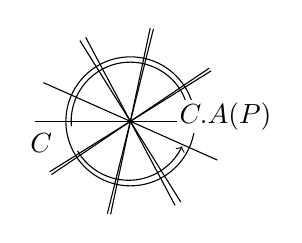
\begin{tikzpicture}[scale=0.78,baseline={(0,0)}]
\draw (0,0) circle (1.05);
\foreach \a in {0,32,76,118,156,214,258,302}
  {\draw ({1.55*cos(\a)},{1.55*sin(\a)})--({-1.55*cos(\a)},{-1.55*sin(\a)});}
\draw[->] (-0.96,-0.08) arc[start angle=185,end angle=15,radius=0.96];
\draw[->] (-0.86,-0.48) arc[start angle=210,end angle=335,radius=0.96];
\node[fill=white,inner sep=1pt] at (-1.45,-0.35) {$C$};
\node[fill=white,inner sep=1pt] at (1.55,0.08) {$C.A(P)$};
\end{tikzpicture}
\tag{1.7.1}
\]

From now on we assume the following condition.

\paragraph{(1.8) Hypothesis.} The chambers are open simplicial cones. Equivalently, every chamber is the set of points with coordinates $>0$ in a suitable basis of $V$.

\paragraph{(1.9.1) Remark.} Let $P$ be an intersection of walls.
\begin{enumerate}[label=(\roman*)]
\item $(V_P,\mcA_P)$ still satisfies (1.8);
\item the set $\mcA^P$ of traces on $P$ of the walls not containing $P$ still satisfies (1.8).
\end{enumerate}
If $\mcA$ is defined by a Weyl group $W$, see the introduction, then $\mcA^P$ is in general no longer of that type.

\paragraph{(1.9.2) Remark.} Hypothesis (1.8) ensures that, if $P$ is an intersection of walls of a chamber $C$, the condition of (1.6) is satisfied. The chamber $C.A(P)$ is therefore defined.

\paragraph{(1.10) Definition.} Two galleries $G$ and $G'$ with the same endpoints are equivalent, written $G\sim G'$, if there exists a sequence of galleries $G=G_0,\ldots,G_n=G'$ ($n\ge0$) such that $G_{j+1}$ is obtained from $G_j$ as follows:
\begin{enumerate}[label=\alph*)]
\item there are decompositions $G_j=E_1FE_2$ and $G_{j+1}=E_1F'E_2$;
\item there is a chamber $C$ and two walls $M,N$ of $C$ such that $F$ and $F'$ are the two minimal galleries from $C$ to $C.A(M\cap N)$.
\end{enumerate}
Composition of galleries, the operations $G\mapsto G^*$ and $G\mapsto -G$, the source and target maps, and the length function are compatible with this equivalence relation and therefore pass to the quotient. We shall generally denote equivalence classes of galleries by lowercase letters. We say that a class $e$ begins, respectively ends, with a class $f$ if there exists $g$ with $e=fg$, respectively $e=gf$.

\paragraph{(1.11) Proposition.} Equivalent galleries cross each wall the same number of times.

\paragraph{(1.12) Proposition.} Two minimal galleries with the same endpoints are equivalent.

Let $G=(C_0,\ldots,C_n)$ and $G'=(C_0,C'_1,\ldots,C'_n)$ have endpoints $A$ and $B$. We argue by induction on the length of the galleries. The case $n=0$ is trivial, and the induction hypothesis permits us to suppose $C_1\ne C'_1$. Let $M$ and $M'$ be the walls separating $A=C_0=C'_0$ from $C_1$ and $C'_1$, and put $C=A.A(M\cap M')$. The walls $M$ and $M'$ separate $A$ from $B$. By reduction to rank two (1.5)(iii), every wall separating $A$ from $C$ also separates $A$ from $B$.

\[
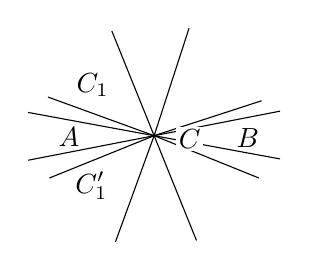
\begin{tikzpicture}[scale=0.82,baseline={(0,0)}]
\coordinate (O) at (0,0);
\foreach \a in {18,72,112,160,202,250,292,338}
  {\draw ({1.75*cos(\a)},{1.75*sin(\a)})--(O);}
\draw (-1.95,-0.38)--(1.95,0.38);
\draw (-1.95,0.36)--(1.95,-0.36);
\node[fill=white,inner sep=1pt] at (-0.95,0.78) {$C_1$};
\node[fill=white,inner sep=1pt] at (-1.32,-0.02) {$A$};
\node[fill=white,inner sep=1pt] at (0.55,-0.05) {$C$};
\node[fill=white,inner sep=1pt] at (1.45,-0.04) {$B$};
\node[fill=white,inner sep=1pt] at (-0.97,-0.78) {$C'_1$};
\end{tikzpicture}
\]
\[
\text{(drawing in }V_{M\cap M'};\ \text{we omit writing }\pi'_{M\cap M'}(\ )\text{).}
\]


Let $F$ (respectively $F'$) be the minimal gallery from $A$ to $C$ passing through $C_1$ (respectively through $C'_1$), and let $E$ be a minimal gallery from $C$ to $B$. The galleries $FE$ and $F'E$ are minimal and equivalent. The minimal galleries $G$ and $FE$, respectively $G'$ and $F'E$, begin with $(A,C_1)$, respectively with $(A,C'_1)$. The induction hypothesis implies that they are equivalent, and (1.12) follows.

\paragraph{(1.13) Notation.} \begin{enumerate}[label=(\roman*)]
\item Let $u(A,B)$ denote the equivalence class of minimal galleries from $A$ to $B$.
\item If $I$ is a set of walls of a chamber $C$, with intersection $P$, put
\[
A(P)=u(C,C.A(P))
\]
(cf. (1.9.2)). If $I$ is the set of all walls, put $A=u(C,-C)$.
\end{enumerate}
The interest of the notation lies in its ambiguity with respect to $C$.

\paragraph{(1.14) Proposition.} Let $A$ be a chamber and let $\mathfrak a$ be a set of gallery classes of bounded length and source $A$. Suppose that $\mathfrak a$ satisfies condition (i):
\begin{enumerate}[label=(i\alph*)]
\item $(A)\in\mathfrak a$;
\item if $gh\in\mathfrak a$, then $g\in\mathfrak a$;
\item let $g$ have target $B$, and let $M,N$ be two walls of $B$. If $gA(M)$ and $gA(N)$ are in $\mathfrak a$, then $gA(M\cap N)$ is in $\mathfrak a$.
\end{enumerate}
Then:
\begin{enumerate}[label=(\roman*)]
\setcounter{enumi}{1}
\item there is a unique gallery class $x$ with source $A$ such that
\[
\mathfrak a=\{g\mid x\text{ begins with }g\}.
\]
\end{enumerate}
Uniqueness is clear: if $x$ begins with $y$ and $x\ne y$, then $y$ has strictly smaller length than $x$. Let $x$ be of maximal length in $\mathfrak a$. To see that it works, it is enough to prove the following assertion:
\[
(*)\quad
\begin{minipage}{0.82\linewidth}
Let $g$ and $M$ be such that (a) $x$ begins with $g$, (b) $x$ does not begin with $gA(M)$, and $gA(M)\in\mathfrak a$. Then there exist $g'$ and $M'$ satisfying again (a) and (b), with $g'$ strictly longer than $g$.
\end{minipage}
\]
Since $gA(M)\in\mathfrak a$, maximality of $x$ implies $g\ne x$, hence $x$ begins with $gA(N)$ for a suitable $N$, necessarily distinct from $M$. By (ic), $gA(M\cap N)\in\mathfrak a$.

Since $gA(M\cap N)$ begins with $gA(M)$, $x$ does not begin with $gA(M\cap N)$. Let $(C_0,\ldots,C_m)$ be the minimal gallery from $A.g$ to $A.gA(M\cap N)$ which begins with $(A.g,A.gA(N))$. Let $i$ ($0<i<m$) be the largest index such that $x$ begins with $g'=g(C_0,\ldots,C_i)$. Then $g'$ and the wall $M'$ between $C_i$ and $C_{i+1}$ satisfy (a)(b).
\[
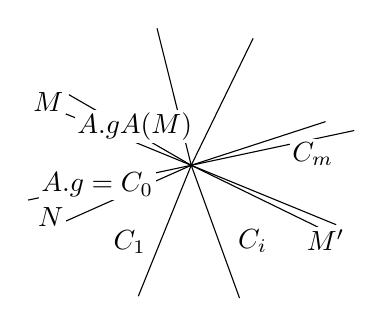
\begin{tikzpicture}[scale=0.92,baseline={(0,0)}]
\coordinate (O) at (0,0);
\foreach \a in {18,64,104,150,204,248,290,334}
  {\draw ({1.95*cos(\a)},{1.95*sin(\a)})--(O);}
\draw (-2.25,-0.48)--(2.25,0.48);
\draw (-2.00,0.82)--(2.00,-0.82);
\node[fill=white,inner sep=1pt,above left] at (-1.72,0.70) {$M$};
\node[fill=white,inner sep=1pt,above] at (-0.78,0.30) {$A.gA(M)$};
\node[fill=white,inner sep=1pt,below left] at (-0.48,-0.06) {$A.g=C_0$};
\node[fill=white,inner sep=1pt,right] at (1.35,0.16) {$C_m$};
\node[fill=white,inner sep=1pt,left] at (-1.72,-0.72) {$N$};
\node[fill=white,inner sep=1pt,below left] at (-0.58,-0.86) {$C_1$};
\node[fill=white,inner sep=1pt,below right] at (0.60,-0.84) {$C_i$};
\node[fill=white,inner sep=1pt,right] at (1.55,-1.03) {$M'$};
\end{tikzpicture}
\]
(projection into $V_{M\cap N}$).

\paragraph{(1.15) Proposition.} Let $A$ be a chamber and let $\mathfrak B$ be a set of chambers. For $\mathfrak B$ to satisfy condition (i):
\begin{enumerate}[label=(i\alph*)]
\item $A\in\mathfrak B$;
\item if $B\in\mathfrak B$, then $D(A,B)\subset\mathfrak B$;
\item let $M,N$ be two walls of a chamber $B$. If $A$ and $B$ are on the same side of $M$ and of $N$, and $B.A(M)$ and $B.A(N)$ belong to $\mathfrak B$, then $B.A(M\cap N)\in\mathfrak B$,
\end{enumerate}
it is necessary and sufficient that:
\begin{enumerate}[label=(\roman*)]
\setcounter{enumi}{1}
\item there exists a unique chamber $C$ such that $\mathfrak B=D(A,C)$.
\end{enumerate}
It is easy to check that (ii) implies (i). To prove the converse, apply (1.14) to the set $\mathfrak a$ of the $u(A,B)$ for $B\in\mathfrak B$, and then apply (1.4)(i) to the gallery class $x=u(A,X)$ obtained.

\paragraph{(1.16) Corollary.} Let $A$ and $B$ be adjacent chambers separated by the wall $M$, and let $C$ be on the same side of $M$ as $B$. There exists $C'$ such that
\[
D(A,C)\cap D_M(B)=D(B,C').
\]

\paragraph{(1.17) Corollary.} \begin{enumerate}[label=(\roman*)]
\item Let $A,C_1,C_2$ be three chambers. There exists $C$ such that
\[
\tag{1.17.1}
D(A,C)=D(A,C_1)\cap D(A,C_2).
\]
\item Let $A$ and $C_1$ be two chambers, and let $M$ be a wall of $A$. There exists $C'$ such that
\[
\tag{1.17.2}
D(A,C')=D(A,C_1)\cap D_M(A).
\]
\end{enumerate}
Indeed, (ii) is the special case of (i) with $C_2=-(A.A(M))$.

\paragraph{(1.18) Lemma.} Let $M,M',M''$ be three distinct walls of a chamber $A$, and put
\[
A_1=A.A(M),\qquad B=A.A(M\cap M'\cap M''),
\]
\[
B'=A.A(M\cap M'),\qquad B''=A.A(M\cap M'').
\]
For any chamber $C$, if $B'\in D(A_1,C)$ and $B''\in D(A_1,C)$, then $B\in D(A_1,C)$.

The facet $F$ of $A$ open in $M\cap M'\cap M''$ is a facet of all the chambers $A,A_1,B,B'$ and $B''$. By (1.5)(iii), we may reduce to the case $\dim V=3$. By (1.17)(ii), we may also suppose that $A_1$ and $C$ are on the same side of $M$. Under these hypotheses, if $B',B''\in D(A_1,C)$, then $M'$ and $M''$ separate $A_1$ from $C$, while $A_1$ and $C$ remain on the same side of $M$. Thus $A$ and $C$ are separated by $M,M'$ and $M''$, and $C=-A=B$.

The following key result is inspired by [4].

\paragraph{(1.19) Proposition.} \begin{enumerate}[label=(\roman*)]
\item Let $A,B,C$ be three chambers, $F$ a gallery from $A$ to $B$, and $G_1,G_2$ two galleries from $B$ to $C$. If $FG_1\sim FG_2$, then $G_1\sim G_2$.
\item Similarly, if $G_1E\sim G_2E$, then $G_1\sim G_2$.
\item Let $g$ be an equivalence class of galleries with source $A$. There exists a chamber $C$ such that $g$ begins with $u(A,B)$ if and only if $B\in D(A,C)$.
\end{enumerate}
Statement (ii) follows from (i) by passing to opposite galleries.

Let $G=(C_0,\ldots,C_n)$ and $G'=(C'_0,\ldots,C'_n)$ be two galleries of length $n$ with the same endpoints. If $n\ge1$, set $G_1=(C_1,\ldots,C_n)$ and $G'_1=(C'_1,\ldots,C'_n)$. If in addition $C_1\ne C'_1$, let $M$ and $M'$ be the walls separating $C_0=C'_0$ from $C_1$ and $C'_1$, and put $A=C_0.A(M\cap M')$.

Consider the following relation $R_n(G,G')$. It means that one of the following holds:
\begin{enumerate}[label=\alph*)]
\item $n=0$;
\item $n\ne0$, $C_1=C'_1$, and $G_1\sim G'_1$;
\item $n\ne0$, $C_1\ne C'_1$, and there exists a gallery $F$ from $A$ to $C_n=C'_n$ such that
\[
G_1\sim u(C_1,A)F,\qquad G'_1\sim u(C'_1,A)F.
\]
\end{enumerate}
We prove by induction on $n$ that $(A_n)$: $R_n$ is an equivalence relation.

Assume $(A_i)$ for $i<n$, and prove the three intermediate assertions below.

\paragraph{(1.19.1)} For galleries of length $i<n$, $R_i(G,G')$ is equivalent to $G\sim G'$.

The implication $R_i(G,G')\Rightarrow G\sim G'$ is trivial, and if $G\sim G'$ then, using the notation of (1.10), one has $R_i(G_j,G_{j+1})$.

\paragraph{(1.19.2)} Assertion (i) is true for composites $FG_i$ of length $<n$. This follows from (1.19.1) and the second clause in the definition of the relations $R_i$.

\paragraph{(1.19.3)} Assertion (iii) is true for $g$ of length $<n$.

This follows from (1.15) applied to the set $\mathfrak B$ of chambers $B$ such that $g$ begins with $u(A,B)$. The hypothesis (ic) of (1.15) is checked using (1.19.2), (1.18), and the third clause in the definition of the $R_i$.

It remains to prove that if $G,G'$ and $G''$ are three galleries of length $n$ from $A$ to $C$, with $R_n(G,G')$ and $R_n(G,G'')$, then $R_n(G',G'')$. If $n=0$, or if $C_1=C'_1$, or if $C_1=C''_1$, this is trivial.

For $n>0$, let $M,M',M''$ be the walls separating $A=C_0=C'_0=C''_0$ from $C_1,C'_1,C''_1$. There are two cases.

\emph{Case 1.} $C_1\ne C'_1=C''_1$. Let $B=A.A(M\cap M')$. By hypothesis,
\[
(C_1,\ldots,C_n)\sim u(C_1,B)F'\sim u(C_1,B)F'',
\]
\[
(C'_1,\ldots,C'_n)\sim u(C'_1,B)F',\qquad
(C''_1,\ldots,C''_n)\sim u(C''_1,B)F''.
\]
By (1.19.2), $F'\sim F''$, hence $R_n(G',G'')$.

\emph{Case 2.} $C_1,C'_1,C''_1$ are pairwise distinct. Put
\[
B_1=A.A(M'\cap M''),\quad B'=A.A(M\cap M'),\quad
B''=A.A(M\cap M''),
\]
and $B=A.A(M\cap M'\cap M'')$. Then
\[
G_1\sim u(C_1,B')F'\sim u(C_1,B'')F'',
\]
\[
G'_1\sim u(C'_1,B')F',\qquad
G''_1\sim u(C''_1,B'')F''.
\]
Thus the class $g_1$ of $G_1$ begins with $u(C_1,B')$ and $u(C_1,B'')$. By (1.19.3) and Lemma (1.18), $g_1$ begins with $u(C_1,B)$:
\[
G_1\sim u(C_1,B)F.
\]
By (1.19.2), $F'\sim u(B',B)F$ and $F''\sim u(B'',B)F$. Hence
\[
G'_1\sim u(C'_1,B)F,\qquad G''_1\sim u(C''_1,B)F.
\]
Therefore
\[
G'_1\sim u(C'_1,B_1)u(B_1,B)F,
\qquad
G''_1\sim u(C''_1,B_1)u(B_1,B)F,
\]
and so $R_n(G',G'')$.
\[
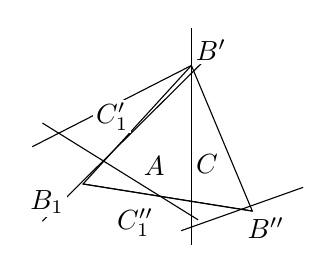
\begin{tikzpicture}[scale=0.86,baseline={(0,0)}]
\coordinate (L) at (-1.25,-0.65);
\coordinate (T) at (0.35,1.10);
\coordinate (R) at (1.25,-1.05);
\draw (L)--(T)--(R)--cycle;
\draw (L)--(R);
\draw (0.35,1.65)--(0.35,-1.55);
\draw (-1.85,-1.20)--(0.85,1.48);
\draw (-2.0,-0.10)--(0.35,1.10);
\draw (-1.85,0.25)--(0.45,-1.18);
\draw (0.20,-1.34)--(2.00,-0.70);
\node[fill=white,inner sep=1pt] at (-1.78,-0.92) {$B_1$};
\node[fill=white,inner sep=1pt] at (-0.82,0.35) {$C'_1$};
\node[fill=white,inner sep=1pt] at (-0.48,-1.22) {$C''_1$};
\node[fill=white,inner sep=1pt] at (-0.20,-0.38) {$A$};
\node[fill=white,inner sep=1pt] at (0.58,-0.36) {$C$};
\node[fill=white,inner sep=1pt] at (0.64,1.32) {$B'$};
\node[fill=white,inner sep=1pt] at (1.45,-1.30) {$B''$};
\end{tikzpicture}
\]
(a drawing on the unit sphere of $V_{M\cap M'\cap M''}$).

\paragraph{(1.20) Corollary.} The conditions (i) and (ii) of (1.14) are equivalent.

Assume (ii) and prove (ic). Under the hypotheses of (ic), if $x=gh$, with $h$ of source $B$, then (1.19)(i) implies that $h$ begins with $A(M)$ and $A(N)$. Let $C$ be the chamber guaranteed by (1.19)(iii) for $h$. Since $M$ and $N$ separate $B$ from $C$, $\pi'_{M\cap N}(C)$ can only be $\pi'_{M\cap N}(B).A$.
\[
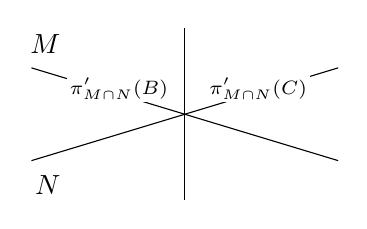
\begin{tikzpicture}[scale=0.95,baseline={(0,0)}]
\draw (-2.05,0.62)--(2.05,-0.62);
\draw (-2.05,-0.62)--(2.05,0.62);
\draw (0,-1.15)--(0,1.15);
\node[fill=white,inner sep=1pt,above left] at (-1.62,0.77) {$M$};
\node[fill=white,inner sep=1pt,below left] at (-1.62,-0.77) {$N$};
\node[fill=white,inner sep=1pt,above] at (-0.88,0.15) {$\scriptstyle\pi'_{M\cap N}(B)$};
\node[fill=white,inner sep=1pt,above] at (0.98,0.15) {$\scriptstyle\pi'_{M\cap N}(C)$};
\end{tikzpicture}
\]
And (ic) follows from (1.5)(iii).

\paragraph{(1.21) Corollary.} For every chamber $A$, let $n(A,i)$ be the number of gallery classes with source $A$ and length $i$. Put
\[
f_A=\sum_{0}^{\infty}n(A,i)t^i\in\Z[[t]].
\]
For every chamber $A$, and for $P$ running through the intersections of walls of $A$, including $\{0\}$ and $V$, one has
\[
\sum_P (-1)^{\codim P}t^{d(A,A.A(P))}f_{A.A(P)}=1.
\]
This expresses the facts that:
\begin{enumerate}[label=\alph*)]
\item the number of gallery classes of length $i$ which begin with $A(P)$ is
\[
n(A.A(P),i-d(A,A.A(P)));
\]
\item gallery classes which begin with both $A(P)$ and $A(Q)$ begin with $A(P\cap Q)$.
\end{enumerate}

\paragraph{(1.22) Algorithm.} Let $G=(A_0,\ldots,A_n)$ be a gallery of length $n>1$, let $G_1=(A_1,\ldots,A_n)$, let $M$ be the wall separating $A_0$ from $A_1$, let $C$ be the chamber whose existence is guaranteed by (1.19)(iii) for $G$, and let $C_1$ be the analogous chamber for $G_1$. One can compute $C$ recursively using the formula
\[
\tag{1.22.1}
D(A_1,C)=D_M(A_1)\cap D(A_1,C_1).
\]
Since $A_1\in D(A,C)$, the wall $M$ separates $A$ from $C$, and $C\in D_M(A_1)$. By (1.19)(i), one also has $D(A_1,C)\subset D(A_1,C_1)$, giving one inclusion. Finally, if $B\in D_M(A_1)\cap D(A_1,C_1)$, then $G_1$ begins with $u(A_1,B)$ and $G$ begins with
\[
u(A,A_1)u(A_1,B)=u(A,B),
\]
which proves (1.22.1).

\paragraph{(1.23) Corollary.} Let $G$ and $H$ be two composable galleries. Let $A$ be the source of $G$, $B$ the source of $H$, and let $C$ be as in (1.19)(iii), so that
\[
H\sim u(B,C)H'.
\]
Then, for every chamber $D$, the class of $GH$ begins with $u(A,D)$ if and only if the class of $Gu(B,C)$ begins with $u(A,D)$.

\end{document}
